\section{Evaluation of LLMs}

The rapid advancement of large language models (LLMs) and their integration into AI chatbots, particularly through Natural Language Generation (NLG) and Retrieval-Augmented Generation (RAG) frameworks, has significantly transformed the landscape of machine-human interaction. These sophisticated systems have become essential tools in various applications due to their ability to generate highly coherent and contextually relevant responses. However, as these models continue to grow in complexity and capability, the need for rigorous and comprehensive evaluation methodologies has become increasingly essential.

Evaluating the performance of LLMs is crucial given their integral role in numerous AI applications that require not only natural language generation but also accurate information retrieval and utilization. As these models are deployed in real-world scenarios, it is imperative to meticulously evaluate their ability to handle diverse inputs, generate accurate and contextually appropriate responses, and adhere to ethical guidelines.

\begin{figure}[h!]
    \centering
    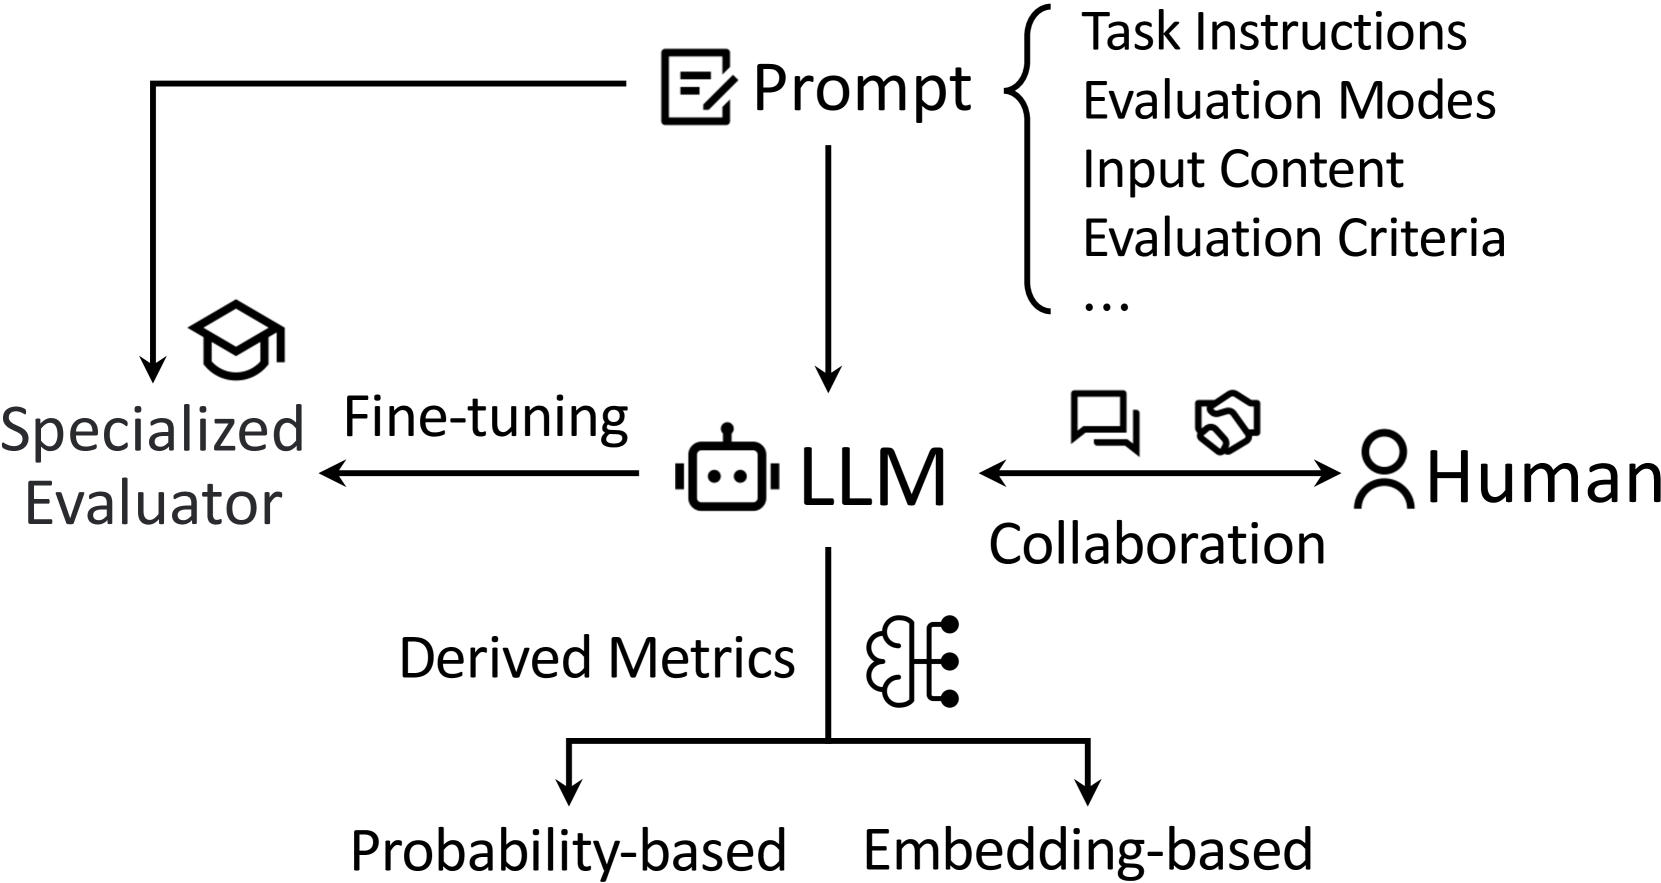
\includegraphics[width=0.8\textwidth]{images/eval/x1.png}
    \caption{A schematic introduction of LLM-based NLG evaluation techniques, that highlights the integration of traditional metrics with advanced LLM-derived methods and human collaboration. \textit{Source:} \cite{gao2024llm}}
    \label{fig:evaluation_pipeline}
\end{figure}

Traditionally, NLG evaluation has relied on surface metrics such as BLEU and ROUGE, which measure the n-gram overlap between generated text and reference texts \cite{papineni2002bleu, lin2004rouge}. Although these metrics are valued for their simplicity and ease of use, they have been criticized for their inability to capture the deeper semantic quality of the text, often leading to low correlation with human judgments \cite{sulem2018bleu}. In contrast, evaluation of RAG systems goes beyond simple text generation and includes the quality of information retrieval, a critical factor in the model's ability to provide accurate and relevant answers.

This chapter provides a comprehensive exploration of evaluation methodologies for LLMs and RAG systems. It delves into various techniques ranging from traditional metrics like BLEU and ROUGE, which offer a surface-level assessment, to more advanced, LLM-derived methods that better capture the nuanced quality of generated text. By highlighting the unique challenges posed by NLG and RAG, as well as the innovative solutions developed to address them, this chapter aims to provide a comprehensive understanding of the strategies necessary to ensure that LLMs are reliable, ethical, and meet the rigorous standards required for real-world applications, such as the AI chatbots. As LLMs continue to evolve, so too must the evaluation frameworks, adapting to maintain their effectiveness across a broad spectrum of tasks and scenarios.

\section{Evaluation of Natural Language Generation (NLG)}

\subsection{Model-Based Evaluation Metrics and NLP Tasks}

The advent of deep learning has led to the development of more sophisticated evaluation metrics for LLMs that go beyond traditional methods such as BLEU and ROUGE. These advanced metrics, such as BERTScore and BARTScore, exploit pre-trained language models to evaluate generated text with a focus on aspects such as fluency, coherence, and fidelity \cite{zhang2019bertscore, yuan2021bartscore}. BERTScore, for example, calculates the similarity between the embeddings of generated and reference texts, providing a more nuanced evaluation than overlapping n-grams. BARTScore further improves this approach by considering the conditional probability of the generated text given the source text, offering indications of the likelihood that a high-quality language model will produce the content \cite{gao2023retrieval}.

Although these model-based metrics represent significant improvements over traditional evaluation methods, they are not without their limitations. One major drawback is their dependence on reference texts, which limits their applicability in scenarios where such references are not available. Moreover, despite being more in line with human judgments, these metrics may still have problems with some aspects of text quality, such as robustness in different contexts and efficiency in the use of computational resources \cite{he2022blind}. These challenges highlight the need for continuous refinement of evaluation techniques to keep pace with the evolving capabilities of LLMs.

In the context of AI chatbots, evaluation of NLP tasks, which include both comprehension and text generation, is indispensable to ensure that these systems can engage users in meaningful interactions. In particular, Natural language generation (NLG) is a crucial aspect of NLP, involving tasks such as summarization, dialogue generation, machine translation, and open-ended text creation. Evaluation of NLG capabilities is vital in AI chatbots field to determine how effectively these models generate appropriate and contextually relevant responses to user input. Specifically, dialogue generation and question answering are paramount, as they form the basis of a chatbot's ability to communicate naturally and provide informative and accurate answers.

\subsubsection{Dialogue Generation}

The evaluation of dialogue generation is essential to developing more intelligent and natural dialogue systems. It involves evaluating the model's ability to understand context, generate consistent responses, and maintain a conversation over multiple shifts. Recent studies have shown that models such as Claude and ChatGPT outperform earlier versions in dialogue tasks, with Claude demonstrating slight advantages in specific configurations \cite{lin2023llm, qin2023chatgpt}. Fine-tuning LLMs for specific tasks has been found to significantly improve performance, with fine-tuned models often outperforming generic models such as ChatGPT in task-oriented, knowledge-based dialogue contexts \cite{bang2023multitask}.

\subsubsection{Question Answering (QA)}

Question Answering is another pivotal task for AI chatbots, particularly in applications such as search engines, intelligent customer service, and specialized QA systems. A chatbot's accuracy and efficiency in answering questions are key indicators of its performance. Recent evaluations have shown that models such as InstructGPT davinci v2 (175B) excel in accuracy, robustness, and correctness in various QA scenarios \cite{ouyang2022training, liang2022holistic}. Although ChatGPT has made great strides in improving its QA capabilities, it still faces challenges in specific benchmarks such as CommonsenseQA and Social IQA, where its cautious approach sometimes leads to denial of answers when information is insufficient. Nevertheless, fine-tuned models such as Vícuna and ChatGPT itself continue to demonstrate outstanding performance in QA tasks, underscoring the importance of task-specific optimization to achieve high accuracy and relevance \cite{bai2024benchmarking}.

Evaluation of NLP tasks, particularly dialogue generation and question answering, is essential to ensure that AI chatbots can interact effectively with users. As LLMs continue to advance, accurately assessing and improving these capabilities will be critical to developing more sophisticated and reliable chatbot systems. In addition, continuous improvement of model-based evaluation metrics is essential to capture the full spectrum of capabilities and challenges posed by these advanced models, ensuring that they meet the rigorous standards required for real-world applications.

\subsection{LLM-Derived Metrics}

The emergence of LLMs such as InstructGPT has significantly transformed the landscape of NLG evaluation \cite{ouyang2022training}. Researchers have increasingly turned to LLM-derived metrics that leverage the linguistic and contextual capabilities of these models to more effectively assess the quality of generated text. These metrics go beyond traditional n-gram-based methods by assessing the semantic similarity between generated and reference texts using embeddings produced by LLMs. For example, OpenAI's text-embedding-ada-002 model measures similarity scores between texts, with higher scores indicating closer alignment with the desired quality of the output \cite{es2023ragas}.

In addition to semantic similarity, probability-based approaches have also been introduced that offer more dynamic and context-aware evaluation. GPTScore, for example, uses customized evaluation templates to guide multiple LLMs in assessing various aspects of NLG, such as fluency and coherence, by calculating the probability of the generated text \cite{fu2023gptscore}. These metrics provide a nuanced understanding of text quality, making them a valuable tool for evaluating LLM outputs.

However, despite the advantages of LLM-derived metrics, they are not without their challenges. One of the main problems is robustness. These metrics can be vulnerable in attack scenarios, where adversary inputs can reveal blind spots that traditional metrics might overlook \cite{he2022blind}. In addition, LLM-derived evaluation methods are computationally intensive and often require significant resources, which may limit their applicability in large-scale evaluations. Another critical issue is fairness. These metrics have been found to have social biases, particularly with regard to sensitive attributes such as race, gender, and age, which can lead to biased assessment results \cite{sun2022bertscore}. These challenges underscore the need for continued research to improve the robustness, efficiency, and fairness of LLM-derived metrics.

\subsection{Prompting LLMs for NLG Evaluation}

As the capabilities of LLMs continue to evolve, so do the methods used to assess their performance in NLG. One innovative approach that has emerged is the use of prompts to directly guide LLMs in assessing their own outputs. This method involves the creation of specific prompts that include task instructions, evaluation criteria, and the text to be evaluated, allowing the LLM to autonomously generate the evaluation results \cite{gao2024llm}. The promise of this approach lies in its ability to replicate human-like evaluation processes, making it a valuable tool for assessing the quality of generated text.

Two common methods in prompt-based assessment are scoring and comparison. In scoring, LLMs evaluate text quality on a scale, a method that has shown strong correlation with human judgments in various NLG tasks, such as summarization and dialogue generation \cite{chiang2023can}. Comparison methods, on the other hand, ask LLMs to choose between two generated texts, often proving more reliable than the absolute score \cite{luo2023chatgpt}. In addition, ranking allows LLMs to sort through multiple texts, providing a broader perspective on their evaluation abilities \cite{ji2023exploring}.

Despite its potential, prompt-based assessment has several limitations. Some studies have highlighted problems such as position bias, in which the order in which texts are presented influences the outcome of the evaluation \cite{wang2023large}. It has also been found that LLMs prefer longer and more verbose responses, sometimes even favoring their own generated outputs over those produced by other models \cite{zheng2024judging, liu2023g}. Moreover, these models showed a tendency to evaluate responses with factual errors more favorably than shorter and grammatically correct responses \cite{wu2023style}. Biases, particularly in scoring high quality summaries and non-Latin languages, such as Chinese and Japanese, continue to be a concern \cite{hada2023large}. These challenges underscore the need to continually refine prompt-based scoring methods to ensure fairness, accuracy, and robustness.

\subsubsection{Automatic Evaluation Methods}

Automated evaluation remains a cornerstone in the evaluation of LLMs and Retrieval-Augmented Generation (RAG) systems due to its efficiency, scalability and objectivity. Compared with human evaluation, automated evaluation does not require intensive human participation, which not only saves time but also reduces the impact of human subjective factors and makes the evaluation process more standardized. By using standard metrics and automated tools, this method facilitates the evaluation of model performance in different tasks with minimal human intervention, thus reducing potential biases and enabling rapid evaluation of large volumes of data.

Based on the literature that adopted automatic evaluation, common metrics in automatic evaluation include accuracy, calibration, fairness, and robustness.

\begin{itemize}
    \item Accuracy is a concept that may vary in different scenarios and is dependent on the specific task at hand. However, accuracy tipically is measured using metrics such as Exact Match (EM), F1 score, and ROUGE, which evaluate how well the model's output aligns with a reference answer \cite{chang2024survey}.
    \item Calibration, on the other hand, assesses the model’s confidence levels, ensuring that the predicted probabilities reflect the actual likelihood of correctness. The most commonly used metric to evaluate model calibration performance is Expected Calibration Error (ECE) \cite{guo2017calibration}.
    \item Fairness metrics evaluate whether the model's performance is consistent across different demographic groups, thereby mitigating potential biases. These metrics include Demographic Parity Difference (DPD) and Equalized Odds Difference (EOD) \cite{wang2023decodingtrust}.
    \item Robustness metrics like Attack Success Rate (ASR) and Performance Drop Rate (PDR) measure the model's resilience to adversarial inputs and out-of-distribution data \cite{zhu2023promptbench}.
\end{itemize}

\begin{table}[h!]
\centering
\begin{tabular}{|l|l|}
\hline
\textbf{General metrics} & \textbf{Metrics} \\ \hline
Accuracy & Exact match, Quasi-exact match, F1 score, ROUGE score \\ \hline
Calibrations & Expected calibration error, Area under the curve \\ \hline
Fairness & Demographic parity difference, Equalized odds difference \\ \hline
Robustness & Attack success rate, Performance drop rate \\ \hline
\end{tabular}
\caption{General metrics and their corresponding evaluation metrics. \textit{Source:} \cite{chang2024survey}}
\end{table}

The increasing sophistication of LLMs has led to the development of advanced automatic evaluation tools such as LLM-EVAL and PandaLM, which offer multidimensional evaluation frameworks that enhance the thoroughness and reproducibility of assessments by training an LLM that serves as the “judge” to evaluate different models \cite{lin2023llm, wang2023pandalm}. These tools are often integrated into benchmarks like MMLU, HELM, C-Eval and  Chatbot Arena, further standardizing the evaluation process across different tasks and domains, thereby providing a more comprehensive picture of LLM performance \cite{chang2024survey}.

\subsubsection{Human Evaluation Methods}

While automatic evaluation provides valuable quantitative insights, there are certain tasks where the nuanced understanding that only human evaluation can offer is indispensable. This is particularly true for open-ended generation tasks, where the subjective quality of the text, including aspects such as fluency, relevance, and alignment with human values, must be assessed. In such cases, embedded similarity metrics like BERTScore may fall short, making human judgment essential \cite{novikova2017we}.

Human evaluation typically involves experts, researchers, or lay users who assess LLM and RAG system outputs based on criteria such as accuracy, relevance, fluency, transparency, safety, and human alignment. These key evaluation metrics are crucial for ensuring the quality and appropriateness of generated content. As introduced in the previous section, accuracy ensures that the generated content is factually correct, while relevance checks whether the output is pertinent to the context or query. Fluency evaluates the readability and coherence of the text, transparency examines the clarity of the model’s decision-making process, safety focuses on avoiding harmful or inappropriate content, and human alignment ensures that the output respects societal norms and user expectations \cite{chang2024survey}.

Moreover, the number of evaluators plays a significant role in ensuring the reliability of the evaluation. As highlighted in Table 4.2, having adequate representation and statistical significance in the number of the evaluators is critical to achieving meaningful results. Additionally, the evaluator’s expertise level, including their relevant domain expertise, task familiarity, and methodological training, directly impacts the evaluation’s accuracy and reliability.

\begin{table}[h!]
\centering
\begin{tabular}{|p{4cm}|p{8cm}|}
\hline
\textbf{Evaluation Criteria} & \textbf{Key Factor} \\ \hline
Number of evaluators & Adequate representation, Statistical significance \\ \hline
Evaluation rubrics & Accuracy, Relevance, Fluency, Transparency, \newline Safety, Human alignment \\ \hline
Evaluator’s expertise level & Relevant domain expertise, Task familiarity, \newline Methodological training \\ \hline
\end{tabular}
\caption{Summary of key factors in human evaluation. \textit{Source:} \cite{chang2024survey}}
\end{table}

However, also human evaluation is not without challenges. It is often resource-intensive, time-consuming and susceptible to variability due to cultural and individual differences among evaluators. Ensuring a representative number of evaluators and defining clear evaluation criteria are critical to mitigating these challenges. Furthermore, the expertise level of the evaluators plays a crucial role in the reliability of the evaluation, particularly in domain-specific tasks where deep subject knowledge is required \cite{chang2024survey}.

Recognizing the strengths and limitations of both LLMs and human evaluators, researchers have proposed a collaborative approach that leverages the best of both worlds. In this hybrid method, LLMs generate initial evaluations, which are then reviewed and refined by human evaluators. This collaborative process has shown promise in reducing the workload of human evaluators while maintaining high accuracy. Techniques like the COEVAL pipeline depicted in Figure \ref{fig:coeval_pipeline} combine LLM-generated evaluations with human scrutiny. This method results in more reliable and nuanced evaluations, particularly for complex or open-ended tasks \cite{li2023collaborative, zhang2021human}.

However, also the collaborative approach is not without its drawbacks. It still requires significant human involvement, which can limit its scalability and cost-effectiveness compared to fully automated methods. As research progresses, it will be crucial to develop unified benchmarks and explore new evaluation scenarios that fully realize the potential of LLMs in NLG evaluation. This evolution in evaluation methods aims to address the persistent challenges of bias, efficiency, and robustness, ensuring that LLMs can be effectively and fairly assessed across diverse applications \cite{gao2023retrieval}.

\begin{figure}[h!]
    \centering
    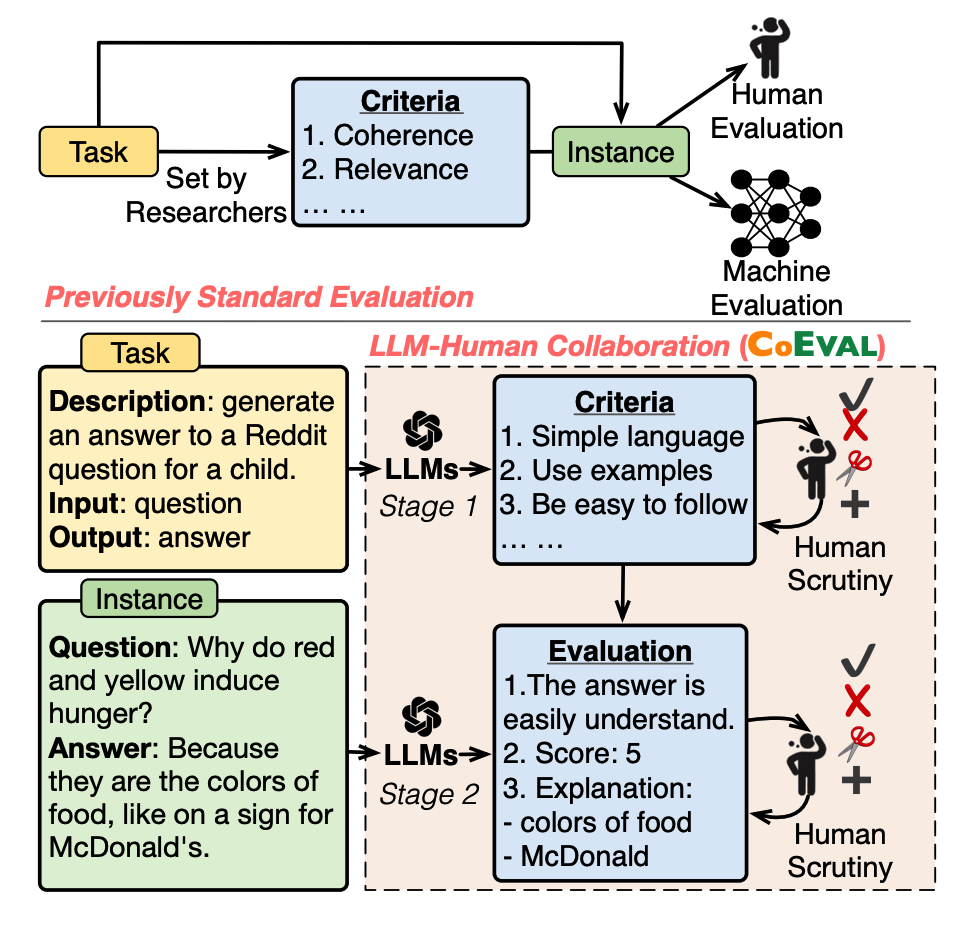
\includegraphics[width=0.5\textwidth]{images/eval/coeval.png}
    \caption{The COEVAL pipeline demonstrates a collaborative evaluation approach, combining LLM-generated ideation with human scrutiny to refine and validate the evaluation process. This method, illustrated in the lower part of the figure, contrasts with conventional evaluation methods (upper part) by integrating both machine-driven and human-refined assessments. \textit{Source:} \cite{li2023collaborative}}
    \label{fig:coeval_pipeline}
\end{figure}

In practice, a combination of automatic and human evaluation methods is often employed to achieve a more comprehensive assessment of chatbot performance. This hybrid approach allows the strengths of both methods to be harnessed, providing a more balanced and thorough evaluation of AI chatbots that use LLMs and RAG technologies. As the field continues to evolve, the integration of these methods will be key to refining evaluation processes and ensuring that AI systems meet the high standards required for real-world applications.

\subsubsection{Evaluation of Factuality, Robustness, and Trustworthiness}

Evaluating the factuality, robustness, trustworthiness, and ethic aspects of AI chatbots that leverage LLMs is essential, particularly as these systems are increasingly deployed in real-world scenarios where they must handle unexpected inputs and adversarial attacks.

\textbf{Factuality:} Beyond the general quality of generated text, the factuality of LLM outputs is a crucial aspect of their evaluation. Factuality refers to the degree to which the information or responses generated by the model align with real-world truths and verifiable facts. This aspect is particularly crucial in applications like AI chatbots, where accuracy and reliability are essential, especially in tasks such as question answering (QA) systems, dialogue systems, information extraction, text summarization, and automated fact-checking.

Errors in the information provided by LLMs can lead to misunderstandings, misinformation, and potentially harmful consequences. Therefore, factuality evaluation involves assessing the model’s ability to remain consistent with known facts, avoid generating misleading or false information, often referred to as "factual hallucination", and effectively learn and recall factual knowledge.

Several methodologies have been proposed to measure and enhance the factuality of LLMs. For instance, Wang et al. conducted an assessment of several large models, including InstructGPT, GPT-3.5, GPT-4, and BingChat, by evaluating their performance in answering open questions. Their study, which involved human evaluation, found that while models like GPT-4 and BingChat provided correct answers for over 80\% of the questions, there remained a significant accuracy gap of over 15\%, indicating that further improvements are necessary to achieve complete factual correctness \cite{wang2024evaluating}.

To improve factuality evaluation methods, Honovich et al. reviewed current approaches and identified a lack of a unified comparison framework. They addressed this by converting existing factual consistency tasks into binary labels that assess whether there is a factual conflict with the input text. This approach, which does not rely on external knowledge such as the RAG framework, has shown that methods based on natural language inference (NLI) and question generation answering can complement each other effectively in evaluating factuality \cite{honovich2022true}.

The TruthfulQA dataset, introduced by Lin et al., has become a widely used tool for evaluating the factuality of LLMs. Designed to challenge models with scenarios where producing factual answers is difficult, TruthfulQA tests the models' ability to remain truthful under challenging conditions. Findings from experiments using TruthfulQA suggest that merely scaling up model sizes does not necessarily improve truthfulness, highlighting the need for more sophisticated training approaches \cite{lin2021truthfulqa}.

The evaluation of factuality in LLMs is a complex but essential task, with significant implications for the reliability and trustworthiness of AI systems that leverage these models. As research progresses, refining these evaluation methods will be critical to ensuring that LLMs can consistently provide accurate and truthful information across a wide range of applications. Simultaneously, ongoing advancements in LLM-derived metrics will continue to play a crucial role in the broader evaluation of NLG capabilities, addressing issues of robustness, efficiency, and fairness. From the discourse presented, it becomes evident that integrating external knowledge, as seen in the RAG framework, offers a viable solution to enhance the factuality of LLMs in NLG.

\textbf{Robustness:} Robustness evaluation focuses on how well AI chatbots handle unexpected or out-of-distribution (OOD) inputs, as well as adversarial prompts designed to manipulate the system \cite{wang2022generalizing}. Robustness is crucial for ensuring that LLMs maintain their performance and reliability even when faced with inputs that deviate from the norm. Early evaluations of models such as ChatGPT revealed potential security risks when these systems were exposed to adversarial inputs or manipulated through visual input, underscoring the need for more resilient models \cite{yang2022glue}. Further studies have shown that contemporary LLMs remain vulnerable to adversarial text attacks at various levels, from character-level perturbations to more complex semantic manipulations \cite{zhu2023promptbench}. These findings highlight the importance of developing models that can withstand diverse and potentially malicious inputs while maintaining their intended functionality.

\textbf{Trustworthiness:} Trustworthiness is another vital aspect of evaluating the performance of AI chatbots. Trustworthiness encompasses the model's ability to provide accurate, ethical, and unbiased responses. This aspect is important for maintaining user trust and ensuring that AI systems are deployed responsibly. Studies such as DecodingTrust have expanded the scope of trustworthiness evaluation to include dimensions like toxicity, stereotype bias, adversarial robustness, and fairness. While advanced models like GPT-4 may show improvements in these areas, they are not immune to certain vulnerabilities, including susceptibility to cognitive biases and ethical inconsistencies. For instance, research has indicated that while LLMs can avoid common cognitive errors, their consistency in judgment can be compromised by factors such as questioning, negation, or misleading cues, raising concerns about their reliability in real-world scenarios \cite{wang2023decodingtrust}.

\textbf{Ethics and Bias:} The ethical implications and biases of AI chatbots are critical areas of evaluation, particularly as these systems are deployed in sensitive or high-stakes environments. LLMs have been found to internalize and perpetuate harmful biases present in their training data, leading to outputs that may include offensive language, hate speech, or stereotypes related to gender, race, religion, and other demographic characteristics. These biases not only compromise the fairness of the system but also pose significant risks in applications where unbiased and equitable interactions are paramount. Recent studies have systematically evaluated the presence of such biases in models like ChatGPT, revealing that despite advancements, these models continue to exhibit toxic and biased content \cite{zhuo2023red}. Moreover, role-playing scenarios have been shown to exacerbate these biases, leading to increased toxicity and biased outputs up to 6 times toward specific entities \cite{deshpande2023toxicity}. These ethical concerns highlight the need for ongoing evaluation and mitigation strategies to ensure that AI chatbots provide equitable and non-discriminatory interactions, fostering trust and minimizing potential harm to users. The topics of ethics and bias, along with strategies for their mitigation, will be covered in detail in Chapter 6.

In conclusion, while refining the evaluation of LLMs in NLG is vital for ensuring their effectiveness across various applications, it’s important to recognize that the RAG framework presents a promising solution to some of the inherent challenges in NLG. However, RAG itself introduces unique complexities that must be carefully evaluated to ensure that both retrieval and generation processes meet the required standards of accuracy, reliability, and relevance.

\section{Evaluation of Retrieval-Augmented Generation (RAG)}

\subsection{RAG-Specific Evaluation Metrics}

The evaluation of Retrieval-Augmented Generation (RAG) systems extends beyond the conventional assessment of text generation to include the aspect of information retrieval. Unlike standard Natural Language Generation (NLG) tasks, RAG systems are evaluated on two primary fronts: retrieval quality and generation quality. 

Retrieval quality refers to the effectiveness of the retriever component within the RAG system in sourcing relevant information from external databases or knowledge bases. Standard metrics from related fields—such as search engines, recommendation systems, and information retrieval systems—are employed to measure the performance of the retrieval module. For instance, precision, recall, and F1 score are commonly used to evaluate how well the retrieved documents or information chunks align with the intended query.

The assessment of generation quality in RAG systems is pivotal for evaluating the model’s ability to produce coherent, relevant, and contextually accurate responses derived from the retrieved content. This aspect of evaluation is critical, as it determines the effectiveness of the model in synthesizing information to generate responses that meet the user's requirements. Generation quality can be categorized based on the nature of the content: unlabeled and labeled. For unlabeled content, the evaluation focuses on ensuring the faithfulness, relevance, and non-harmfulness of the generated responses, thereby guaranteeing that the output is both meaningful and safe. In contrast, labeled content evaluation emphasizes the accuracy of the information produced by the model \cite{gao2023retrieval}.

Contemporary evaluation methodologies for RAG models emphasize three primary quality scores—context relevance, answer faithfulness, and answer relevance—alongside four essential abilities that collectively inform the evaluation process.

\begin{itemize}
    \item \textbf{Quality Scores:} Quality scores evaluate the efficiency of the RAG model from different perspectives in the process of information retrieval and generation. 
    \begin{itemize}
        \item \textit{Context Relevance} assesses the precision and specificity of the retrieved context, ensuring that the content is directly pertinent to the query while minimizing extraneous information, thus reducing processing overheads.
        \item \textit{Answer Faithfulness} evaluates whether the generated responses remain true to the retrieved context, maintaining consistency and avoiding contradictions in the output.
        \item \textit{Answer Relevance} ensures that the generated responses directly address the posed questions, thereby effectively meeting the user's inquiry with pertinent information \cite{es2023ragas, saad2023ares}.
    \end{itemize}

    \item \textbf{Required Abilities:} The following abilities are critical for the model’s performance under complex scenarios, impacting the quality scores.
    \begin{itemize}
        \item \textit{Noise Robustness} evaluates the model’s capacity to handle noisy or irrelevant documents that may be loosely related to the query but do not provide substantial information. This ability is crucial for filtering out distractions and focusing on high-quality data.
        \item \textit{Negative Rejection} assesses the model’s discernment in refraining from generating a response when the retrieved documents do not contain the requisite knowledge to answer the query, thereby preventing the propagation of misinformation.
        \item \textit{Information Integration} measures the model’s proficiency in synthesizing information from multiple documents to formulate a comprehensive response to complex queries, demonstrating its capability to aggregate and process diverse sources.
        \item \textit{Counterfactual Robustness} tests the model’s ability to recognize and disregard known inaccuracies within documents, ensuring that it does not disseminate misinformation even when confronted with misleading content \cite{chen2024benchmarking, liu2023recall}.
    \end{itemize}
\end{itemize}

These metrics and abilities provide a comprehensive framework for the evaluation of generation quality in RAG systems, ensuring that the model not only generates text aligned with the retrieved data but also directly and accurately addresses the user’s queries. Such evaluation is indispensable for determining the overall effectiveness of RAG systems in practical applications such as AI chatbots, where the retrieval and integration of accurate information are essential. A practical implementation of some of the seen metrics will be presented in Section 5.2.1.

It is important to recognize that while these metrics, derived from extant literature, provide valuable insights, they do not yet constitute a mature or standardized approach for quantifying RAG evaluation aspects. Custom metrics tailored to the specific nuances of RAG models, although not discussed herein, have also been developed in some evaluation studies to address particular challenges.

\subsection{Challenges in RAG Evaluation}

Evaluating RAG systems presents unique challenges that go beyond those encountered in traditional NLG evaluation. One significant challenge is managing noise in the retrieved documents. RAG systems must effectively filter out irrelevant or misleading information to prevent it from degrading the quality of the generated responses. This requires robust noise management techniques that enable the system to disregard extraneous data and focus on the most pertinent information \cite{gao2023retrieval}.

Another challenge is information integration, particularly in scenarios involving multi-hop question answering, where the system must synthesize information from multiple sources to construct a coherent and accurate response. This task is especially complex when the information from different sources is contradictory or incomplete, necessitating advanced techniques for integrating and validating the information before it is used in the generation process \cite{luo2023divide}.

Additionally, RAG systems must exhibit counterfactual robustness, which involves recognizing and disregarding known inaccuracies within the retrieved documents. This is essential to prevent the propagation of incorrect information, especially in contexts where the reliability of the generated content is paramount. The ability to filter out or correct inaccurate data, even when presented as potential answers, is a pivotal aspect of ensuring the trustworthiness and accuracy of RAG-generated content \cite{lewis2020retrieval}.

\section{Benchmarks for LLM and RAG Systems}

The evaluation of AI chatbots that leverage LLMs and RAG systems requires comprehensive benchmarks that assess their performance across a variety of tasks. This section introduces the benchmarks used for general tasks, specific downstream tasks such as question answering, and multi-modal tasks, which are essential for evaluating the holistic performance of these models.

\subsection{Benchmarks for General Tasks}

LLMs are designed to handle a wide array of tasks, making it crucial to evaluate their performance across multiple dimensions. Benchmarks like Chatbot Arena \cite{lmsys2024arena} and MT-Bench \cite{zheng2024judging} play a significant role in this regard. Chatbot Arena offers a platform where users can interact with anonymous chatbot models, casting votes based on their experiences. This real-world engagement allows for the assessment of chatbot models in practical settings, providing valuable insights into their strengths and limitations. Similarly, MT-Bench focuses on evaluating LLMs in multi-turn dialogues, which are essential for simulating realistic conversational scenarios. This benchmark is particularly useful for understanding how well a chatbot can manage extended interactions, a critical aspect of NLP tasks.

Additionally, benchmarks such as HELM \cite{liang2022holistic} and DynaBench \cite{kiela2021dynabench} provide a broader evaluation of LLMs across various NLP tasks, including language comprehension and robustness to adversarial inputs. HELM offers a comprehensive assessment of LLMs' language understanding capabilities, while DynaBench supports dynamic benchmark testing, exploring the effects of distributional shifts and model robustness in interactive settings. These benchmarks contribute to a more nuanced understanding of LLM performance, especially in diverse and challenging scenarios.

\subsection{Benchmarks for Specific Downstream Tasks}

While general benchmarks provide an overarching view of LLM performance, specific downstream tasks require more focused evaluation. Question-answering benchmarks, such as MultiMedQA and FRESHQA, assess how effectively a chatbot can retrieve and generate accurate answers. MultiMedQA, for instance, focuses on medical questions, evaluating a model's clinical knowledge and ability to handle complex queries in the healthcare domain. FRESHQA, on the other hand, tests the chatbot's ability to incorporate up-to-date information from current world knowledge, ensuring relevance and accuracy in dynamic environments \cite{singhal2022large, vu2023freshllms}.

For more complex dialogue and reasoning tasks, benchmarks like Dialogue CoT and ARB provide targeted assessments. Dialogue CoT evaluates LLMs' capabilities in conducting coherent and contextually relevant conversations, while ARB probes their performance in advanced reasoning tasks that span multiple domains. These benchmarks are instrumental in understanding how well LLMs can perform in specialized and challenging tasks that go beyond basic question answering \cite{wang2023cue, sawada2023arb}.

\subsection{Benchmarks for Multi-modal Tasks}

In the evolving landscape of AI, chatbots are increasingly required to handle multi-modal inputs, such as images, text, and even audio. Evaluating these capabilities necessitates benchmarks specifically designed for multi-modal tasks. MME and MMBench are two such benchmarks that rigorously assess the perceptual and cognitive abilities of Multi-modal Large Language Models (MLLMs). MME uses instruction-answer pairs to evaluate models under controlled conditions, while MMBench offers a comprehensive dataset for evaluating vision-language models \cite{yin2023survey, liu2023mmbench}.

These benchmarks ensure that MLLMs are not only capable of understanding and generating text but can also effectively interpret and respond to visual inputs. As MLLMs continue to evolve, benchmarks like SEED-Bench further extend their evaluation to cover a wide range of tasks, including pattern recognition in images and videos, providing a holistic assessment of multi-modal language models \cite{li2023seed}. \newline

The development of robust and comprehensive benchmarks is essential for advancing the evaluation of AI chatbots that utilize LLMs and RAG systems. These benchmarks enable researchers and developers to systematically assess and improve the performance of chatbots across general tasks, specific downstream tasks, and multi-modal tasks. As AI technology continues to progress, these benchmarks will play a critical role in ensuring that chatbots can meet the diverse and complex demands of real-world applications.

\section{Success and Failure Cases of LLMs}

Large Language Models (LLMs) have demonstrated remarkable capabilities across a wide range of tasks, yet they are not without limitations. Understanding both their strengths and weaknesses is essential for evaluating the performance of AI chatbots, particularly in generating dialogue and answering questions.

One of the primary strengths of LLMs lies in their ability to generate text with a high degree of fluency and precision. This capability is evident in tasks such as machine translation, text generation, and question answering, where LLMs consistently produce coherent and contextually appropriate responses.

In addition to text generation, LLMs excel in language understanding tasks. They perform impressively in sentiment analysis, text classification, and handling factual input, showcasing their ability to comprehend and process natural language effectively. Furthermore, LLMs demonstrate robust arithmetic and logical reasoning capabilities, making them well-suited for tasks that require complex calculations or structured data inference. Their proficiency extends to temporal reasoning, where they can accurately interpret and manage time-related information.

The robust contextual comprehension of LLMs enables them to generate responses that are not only accurate but also align well with the input provided, making them effective in dialogue systems and conversational AI.

Despite these strengths, LLMs also exhibit several notable limitations that can affect their performance in certain contexts. One of the primary challenges LLMs face is in tasks requiring nuanced understanding, such as Natural Language Inference (NLI). Here, they struggle to accurately represent human disagreements and may perform poorly in discerning subtle semantic similarities between events. This limitation extends to abstract reasoning, where LLMs often encounter confusion or errors, particularly in complex or ambiguous contexts.

LLMs also demonstrate suboptimal performance when processing linguistic contexts that involve non-Latin scripts or are resource-constrained. Their ability to generate accurate and contextually relevant outputs diminishes significantly in these scenarios, highlighting a gap in their linguistic capabilities across diverse languages and writing systems.

Moreover, LLMs are not immune to the biases and toxic content embedded in the vast datasets on which they are trained. They can inadvertently assimilate and propagate offensive or biased language, which poses significant ethical concerns, particularly in sensitive applications such as social media moderation or customer service.

Another critical limitation of LLMs is their difficulty in incorporating real-time or dynamic information. This makes them less effective in tasks that require up-to-date knowledge or the ability to rapidly adapt to changing circumstances. Additionally, LLMs are particularly vulnerable to adversarial prompts, which can exploit weaknesses in their training and result in incorrect or harmful outputs \cite{chang2024survey}.

Understanding these success and failure cases is crucial for effectively deploying LLMs in real-world applications. By recognizing where LLMs excel and where they fall short, developers and researchers can better design evaluation frameworks that ensure AI chatbots perform reliably and ethically across a wide range of tasks.

\section{Conclusions and Future Directions}

The evaluation of large language models (LLMs) within natural language generation (NLG) and retrieval augmented generation (RAG) systems is a dynamic and rapidly evolving area of research. Traditional evaluation metrics, such as BLEU and ROUGE, have historically laid the foundation for the evaluation of language models. However, as LLMs have progressed, assessment methodologies have evolved, leading to the introduction of sophisticated metrics derived from LLMs such as BERTScore and GPTScore. These advanced metrics facilitate more nuanced evaluations that transcend surface comparisons, offering insights into crucial aspects of text quality such as fluency, coherence, and faithfulness, essential elements for accurate, human-aligned evaluations.

Despite these advances, significant challenges persist, particularly in the evaluation of RAG systems. The complexities of managing noise in retrieved data, synthesizing information from multiple sources, and ensuring counterfactual robustness underscore the need for specialized evaluation tools. As RAG systems become an increasingly integral part of advanced AI applications, it will be critical to develop metrics that accurately reflect these complexities.

Looking forward, the development of unified benchmarks tailored to the distinct needs of NLG and RAG systems will be imperative. Such benchmarks will foster more consistent and comprehensive assessments across different tasks and domains, ultimately contributing to the creation of more reliable and versatile AI systems. In addition, exploring new assessment scenarios, particularly those involving low-resource languages and complex tasks, is essential to unlocking the full potential of LLMs. These scenarios often present unique challenges that are not adequately captured by current frameworks, necessitating the development of more nuanced and context-aware metrics.

The future of LLM evaluation lies in improving collaborative frameworks that combine human judgment with automated methods. By leveraging the strengths of both, researchers can develop evaluation systems that ensure that LLMs provide accurate, fair, and contextually relevant results across a broad spectrum of applications. This hybrid approach has the potential to mitigate the inherent limitations of human and automated assessments, leading to more balanced and reliable evaluations.

A crucial challenge in the evaluation of LLMs is the need for comprehensive behavioral assessment. As artificial intelligence systems approach the threshold of artificial general intelligence (AGI), it becomes increasingly important to assess their behavior in open, real-world environments. This involves not only evaluating their performance on specific tasks, but also understanding their decision-making processes and their adaptability to dynamic scenarios. Incorporating multimodal dimensions into these assessments, where LLMs are evaluated as central controllers in complex systems such as robotics, could provide a more holistic understanding of their capabilities.

In addition, the dynamic and evolving nature of LLMs presents a challenge to traditional static evaluation protocols. As these models continue to improve, there is a risk that they will become too familiar with existing benchmarks, leading to inflated performance metrics that do not accurately reflect their capabilities in the real world. To solve this problem, future evaluation systems must be dynamic and able to evolve along with the models they evaluate. This could involve creating adaptive benchmarks that evolve over time or implementing real-time evaluation methods that continuously test models with new and unseen data.

In conclusion, the field of LLM evaluation is at a crucial stage, with significant opportunities to advance the understanding and evaluation of these powerful models. By addressing the challenges of comprehensive behavioral assessment, robustness, and dynamic evaluation, researchers can ensure that LLMs continue to improve in meaningful and measurable ways. As LLMs become increasingly integral to a wide range of applications, the development of more comprehensive and forward-looking evaluation methodologies will be crucial to driving the continued success and ethical deployment of AI technologies.
